% Chapter 2

\chapter{Basics} % Main chapter title

\label{Chapter2} % For referencing the chapter elsewhere, use \ref{Chapter2} 

This chapter introduces the concept of \emph{Software Integration} and \emph{Software Delivery} used in modern Software Development. Section~\ref{section:Softwareconfigurationmanagement} highlights the key importance of \ac{SCM} and why versioning software packages is among the industry best practices. The chapter highlights keywords like \emph{Application and Product release cycle} and is intended to
answer the following question.

\vspace{0.5cm}
\noindent Question 1: What is Software Integration and Delivery and why is this concept so important in the field of Software Development?
\vspace{0.5cm}


\noindent The main goal of this chapter is to deliver a feature process that is capable of fulfilling the concept of Software Integration and Delivery without any manual intervention. The second part of the chapter (section~\ref{section:embeddedlinux}) outlines the basics of Embedded Linux distribution with reference to the Yocto project, Poky, OpenEmbedded build system, metadata, BitBake, and recipes. 
%----------------------------------------------------------------------------------------

\section{Software Integration}\label{section:SoftwareIntegration}
The concept of \keyword{Software Integration} is defined by the process of bringing software packages and applications to work closely with one another and extending its functionalities to the fullest potential without hindering its quality. It has multiple use cases and advantageous in terms of better software productivity and offers better quality. The past decade has witnessed a surge in software development and some significant changes in terms of integration and deployment of software packages. In today’s world, the culture of DevOps is integrated into projects which brings in automation to application build and test and key features like versioning each software packages. This ultimately improves the product and software release lifecycle and provide a better software quality.    

\subsection{Software Configuration Management} \label{section:Softwareconfigurationmanagement}

In contrast to software integration, \ac{SCM} is a quintessential part, which gives stakeholders \footnote{Stakeholders: Development Team, Testers, Customers, Project Managers} the ability to track or control changes to a given software package with the help of \emph{revision control} or \emph{version control}. It helps to identify all the code changes, improvements and bug fixes committed to a project. Software package release versions are determined by a unique version number. Mostly the version numbers are in the form x.y.z(where all three version components are positive integers) and tracks major changes:minor changes:patch updates committed to the software package. Package releases version number in the $[1.0.0; +\infty]$ range are denoted as \emph{production releases} \footnote{From semver FAQ, Software packages used in production should already be 1.0.0~\parencite{preston2013semantic}, also defined as public API} while package releases with a version number in the $[0.0.0;1.0.0]$ version range are called \emph{initial development releases}~\parencite{8721084}.

%----------------------------------------------------------------------------------------
\subsection{Software Integration}
\label{section:applicationsoftwareintegration}
Beyond the concept of software configuration management, Software Integration process includes many stages, building the source code, compiling it, integration testing, system testing, deployment, operations, among others. Software integration and automation have been the areas of key concern in software engineering~\parencite{vasilescu2015quality}. Software integration at the application level starts with the build stage. Here, the source code is checked out from the source code management repository via \emph{Webhooks} or manual run, compiling the application inside the build environment (\emph{Docker containers} are the best use case here), running unit test to test the application and finally moves to the software delivery or the deployment stage.

The process of Software integration have been further boosted by the introduction of \emph{\ac{CI})} approach (see figure \ref{fig:Continuous Integration approach}) where the build is triggered, when there is a commit to the source code repository. The compilation and testing stages are all automated via a \ac{CI} pipeline. With the help of \ac{CI} server like Jenkins, software development can be further streamlined~\parencite{smart2011jenkins}. In the context of software development, \ac{CI} is meant to prevent the “it works on my machine”  syndrome  before  the  code hits production~\parencite{6802994}.

\begin{figure}[H]
\centering{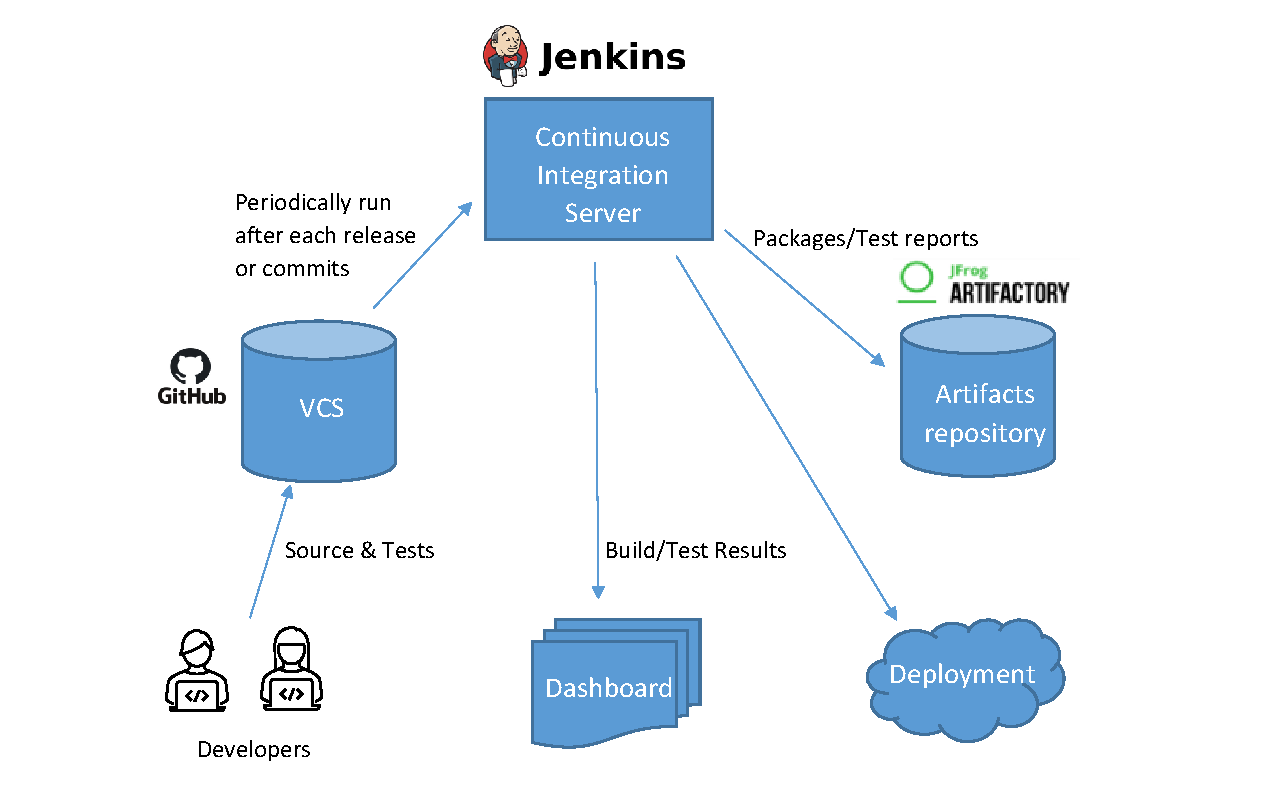
\includegraphics[width=1\textwidth]{figures/SoftwareIntegration.pdf} }%
\caption[Continuous Integration approach]{The Continuous Integration approach\footnotemark}
\label{fig:Continuous Integration approach}
\end{figure}


\footnotetext{Reference image "A typical software process using a \ac{CI} approach." taken from \parencite[p-4]{ant}. In this figure, VCS refers to Version Control System}

%----------------------------------------------------------------------------------------
\section{Software Delivery}\label{section:SoftwareDelivery}

The term \keyword{Software Delivery} in IT defines a complete phase where software components get all the updates, fixes, features delivered to customer or clients securely and hassle free. It might be confusing for the readers to contemplate which exact software components are being delivered. In reference to the thesis work, software applications or product images, developed within the department is referred as the term "software components". To understand this concept of Software Delivery in a better way, consider the process of software development within Bosch. The initial phase involves requirement analysis and development. Once the development phase is completed, the software components go through quality assurance test and operations before the actual delivery to the customer. The approach of testing software applications or components is vital to the software quality but if maintained in a traditional way, the delivery takes time and also involves manual effort. Often the delivery time of these applications or products gets delayed. So, almost companies over the world including BOSCH Group, have welcomed the idea of modern delivery technique. In other words, it can also be referred as "Continuous Delivery and Deployment”. In a precise way, the term Continuous Deployment means that each commit to the repository is automatically released to production. With Continuous Delivery, each commit ends up with a release candidate, allowing production release to be done manually~\parencite{leszko2017continuous}.

The next few sections will throw light on the traditional delivery approach and its shortcomings and why the modern software delivery technique have welcomed the idea of continuous delivery and deployment of products and software applications. 


\subsection{Traditional delivery process}

Software applications and products have release cycle defined within projects which starts off with the requirement stage, followed by development, quality strategy and lastly operations. This delivery process takes considerable amount of time due to the involvement of manual QA (\ac{UAT}, Integration testing and various other non-functional testing). An error detected by the tester at QA stage has to be passed on to the development stage again, to get it fixed by the developer and then roll back to the QA stage to test the same features. This process have multiple shortcomings as it lacks automation and also the delivery process becomes comparatively slow and requires effective communication between the teams.

\subsection{Modern delivery process}

Modern delivery process is all about fulfilling the shortcomings of traditional approaches of software delivery by bringing in automation into projects and introducing \emph{automated delivery pipeline} or \emph{continuous delivery}~\parencite{leszko2017continuous}. It simply means that with each bug fixes or code changes, the delivery timeline or the application release cycle or the product release cycle doesn't gets hampered.The most accurate definition of continuous delivery is stated by Jez Humble and reads as follows~\parencite{leszko2017continuous}:
\vspace{0.5cm}


\enquote{\emph{Continuous Delivery is the ability to get changes of all types-including new features, configuration changes, bug fixes, and experiments-into production, or into the hands of users, safely and quickly in a sustainable way.}}


\vspace{0.5cm} 

With continuous delivery, the software package or the application is deployed continuously into artifact repository against a development release version or to production.

For example, the DevOps (indicated by the orange block in figure \ref{fig:DevOps model}) model is highly valued in the industry. It combines the entire operations and QA tasks into an automated software delivery pipeline that can be handled by the development team itself~\parencite{leszko2017continuous}. DevOps tools like Jenkins, GitHub and technologies like containers and Kubernetes offers flexibility according to the organizational needs. The overall continuous delivery approach reduces lot of time and error-prone manual effort by bringing in automation into the delivery process of software or product.
\begin{figure}[H]
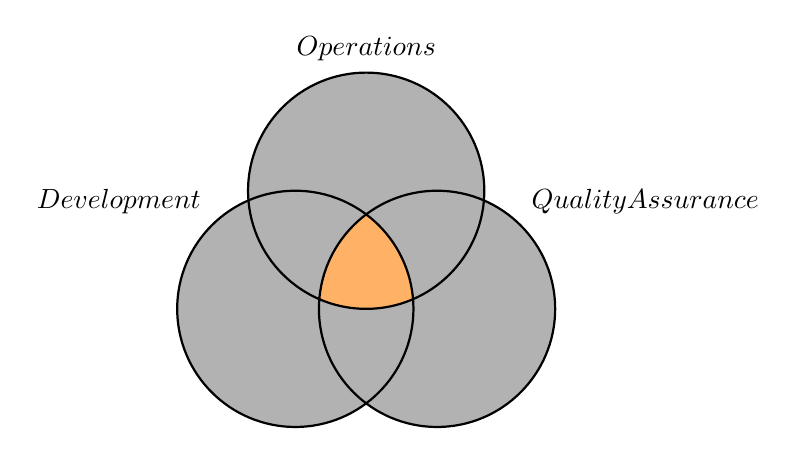
\begin{tikzpicture}[thick,
    set/.style = {circle,
        minimum size = 3cm,
        fill=black!30}]
 
% Set A
\node[set,label={135:$Development$}] (A) at (0,0) {};
 
% Set B
\node[set,label={45:$Quality Assurance$}] (B) at (1.8,0) {};
 
% Set C
\node[set,label=$Operations$] (C) at (0.9,1.5) {};

% Intersection
\begin{scope}
    \clip (0,0) circle(1.5cm);
    \clip (1.8,0) circle(1.5cm);
    \clip (0.9,1.5) circle(1.5cm);
    \fill[orange!60](0,0) circle(1.5cm);
\end{scope}
 
% Circles outline
\draw (0,0) circle(1.5cm);
\draw (1.8,0) circle(1.5cm);
\draw (0.9,1.5) circle(1.5cm);
 
\end{tikzpicture}
\caption[DevOps model]{The DevOps model\footnotemark}
\label{fig:DevOps model}
\end{figure}


The initial phase of the research work also works on the implementation of the \ac{CI} pipeline of the Rest API application used within the department and delivery or deployment pipeline to generate the test reports. The development was carried on the Jenkins server, where the source code was pulled from Git version control and creating a build environment using the Docker container and deploying into Jfrog artifact repository.

\footnotetext{Impression of the reference DevOps model taken from source~\parencite[p-21]{leszko2017continuous}}

%----------------------------------------------------------------------------------------
\section{Software Integration and Software Delivery at a Product level}\label{section:SoftwareIntegrationDeliveryProductLevel}

The end goal of the Yocto project implementation for the target product is to receive all the deliverables packaged into a single delivery location or an output folder. Among other deliverables, the delivery package  includes the Linux \ac{OS} image which is ready to be flashed into the embedded device, integrated with all the required software packages and dependencies. The product image should have a ready-to-use root filesystem for the target. It can be made up of one or more filesystems and may include other artifacts to be available during its generation, such as the Linux kernel, device tree, and bootloader binaries~\parencite{salvador2014embedded}. 

In order to facilitate the process of software integration at ease within the department, the software components included in the Yocto image are continuously integrated via an automated integration pipeline or precisely, the Jenkins pipeline. This evades the manual effort of setting up a physical build host system. At first, the Yocto build repository is hosted with the Git version control tool, which includes the necessary manifest files. A \emph{manifest} file contains the source information about layers or in simple terms, the information about repositories which contains all the \emph{configuration files}, \emph{recipes}, and \emph{class files}. Yocto layers name often prepends \emph{"meta-"} to the front of the layer name.

The high-level view of how the software components get integrated into the product image during the build process is via \emph{Yocto recipes} and layers. These recipes are files that hold information about the source \ac{URL} of the software package and how to fetch a particular software within the build. One can also influence the build by adding software release version numbers in the recipe file. This is always a best practice, as the version specified in the recipe file will fetch the exact software package with a similar version number. Yocto recipes follow a standard naming convention for adding versions with the package name. The process of installation of software package in the Yocto build system is explained in depth in section~\ref{section:softwarepackageinrecipes}. The addition of version helps the product \emph{release cycle}, as tracking changes becomes easier. The entire  lifecycle of a product gets improved. 


With continuous integration of the software packages, software accuracy is reached at better level and the overall deployment time of the product image becomes faster. After the final deployment stage, when the image is mounted on the target hardware, the developer have the possibility to check the software versions via \ac{GUI} or \ac{CLI} of the custom Linux \ac{OS}, which is indeed helpful.

%----------------------------------------------------------------------------------------
\section{The Embedded Linux Landscape}\label{section:embeddedlinux}

When developing an embedded operating system, there are certain criteria’s which a developer should consider.  Firstly, the target hardware is constraint of memory and space. Secondly, the microcontroller’s CPU will be much weaker in comparison to big office machines or even personal computer. So, the operating system should not only be space efficient but also deliver real time operations. The OS is notably the most crucial part of the software adaptation, which  provides abstraction from the hardware through its libraries and application programming interfaces (API)~\parencite{Reference1}. Linux OS for embedded system development is the best choice for developers due to multiple benefits. It is open-source software with lot of support for customization and most importantly the OS image size is small. For example, the Alpine Linux is only 5 MB in size. To classify broadly, there are some generic embedded OS like \keyword{Android} to primarily target mobile phones hardware or \keyword{OpenWrt} to target routers or modems. But mostly, companies build its own custom embedded Linux OS with a set of development tools, specifically designed for a hardware. The thesis work was also carried out on a custom Linux distribution build specially for a particular project specific hardware.

%----------------------------------------------------------------------------------------
\subsection{The Yocto Project}

As perfectly explained in the Yocto project manual~\parencite{Reference2}:
\vspace{0.5cm}


\enquote{\emph{The Yocto Project is an open source collaboration project that helps developers create custom Linux-based systems that are designed for embedded products regardless of the product’s hardware architecture.}}
\vspace{0.5cm}

It is a challenge for developers to build an embedded Linux image from scratch with no pre-build tools or software. The task of building a Linux kernel, a cross-compiler to compile the filesystem and package dependencies is extremely complex and painful. The Yocto project has simplified the process, it has many available software tools and resources to build a hardware independent custom Linux distribution image. It provides flexibility and support multiple customization depending on the project requirement. For example, the Linux distribution or the build system to support a Smart home embedded device may be different to the Linux distribution meant for more complex systems. With the OpenEmbedded build system as the heart of the Yocto project, all the necessary native utilities are build along with software packages by the build engine, BitBake. Bitbake processes the recipe files to define how the software packages should be build. The initial build is comparatively long, but the intermediate build stages use the \ac{SSTATE} cache mechanism that allow reuse of sstate files and this accelerates the build process. Refer to section~\ref{section:bitbake} and section~\ref{section:recipes} for more detailed description of BitBake and Yocto recipe files. 

\begin{figure}[H]
\begin{tikzpicture}
\begin{scope}[xshift=5.5cm]
\coordinate (O) at (0,0);
\draw[fill=red!30] (O) circle (2.8);
\draw[fill=green!40] (O) circle (2);
\draw[fill=yellow!70] (O) circle (1.2);

\draw[decoration={text along path,reverse path,text align={align=center},text={Poky}},decorate] (0.5,0) arc (0:180:0.5);
\draw[decoration={text along path,reverse path,text align={align=center},text={OpenEmbedded build}},decorate] (1.3,0) arc (0:180:1.3);
\draw[decoration={text along path,reverse path,text align={align=center},text={The Yocto Project}},decorate] (2.1,0) arc (0:180:2.1);
%\draw[decoration={text along path,reverse path,text align={align=center},text={Hello, how are you?}},decorate] (2.9,0) arc (0:180:2.9);
\end{scope}
\draw[draw=none] (2.6,0) -- (3.0,0);
\end{tikzpicture}
\caption[The Yocto Project family]{The Yocto Project family}
\label{fig:The Yocto Project family}
\end{figure}


The Yocto Project combines multiple projects under one umbrella. The OpenEmbedded project is the most prominent one. It is the build framework for developing the custom Linux distribution.The OpenEmbedded build system includes \emph{BitBake}, the \emph{OpenEmbedded core} and the reference distribution \emph{Poky}~\parencite{Reference1}.
%----------------------------------------------------------------------------------------

\subsection{Poky}

\emph{OpenedHand},an embedded Linux startup company developed Poky Linux, the Linux distribution build with OpenEmbedded for mobile device~\parencite{Reference1}. Poky offers a cross-compilation environment with the help of BitBake , OE-core layer, and set of metadata~\parencite{salvador2014embedded}. It simplifies the process of configuring the Linux image for the target embedded device by providing a set of blueprints by combining multiple open-source projects for pre-configured embedded Linux OS stacks, and adapt or modify these blueprints to bootstrap the actual system development. At the starting phase of the development project, a Source directory is essential which can be fulfilled by cloning the Poky git repository. The \emph{SOURCE DIRECTORY} includes the recipes, metadata, documentation. Refer below to the following tree structure.
\vspace{0.5cm}
\begin{figure}[H]
\par\noindent
  \centering 
\begin{forest}
  pic dir tree,
  where level=0{}{% folder icons by default; override using file for file icons
    directory,
  },
  [SOURCE DIRECTORY
    [Yocto
    [Poky
        [bitbake]
        [metadata]
        [documentation]
        [LICENSE, file]
        [README, file]
    ]
    ]
  ]
\end{forest}
\end{figure}
\vspace{0.1cm}

With Poky, a custom and intuitive Linux distribution can be build to support different hardware platforms or architecture.

\begin{figure}[H]
\centering
\begin{tikzpicture}[block/.style={regular polygon,regular polygon sides=4,
    inner xsep=2em,align=left,text width=5em,draw},font=\sffamily,thick,
    box/.style={draw,align=left,inner sep=2em},>=stealth
  ]
 \begin{scope}[local bounding box=blocks]
  \node[block] (B1) {OE-Core(meta)};
  \path let \p1=($(B1.east)-(B1.west)$) in 
  node[right=4em of B1,block] (B2) {meta-yocto (Yocto specific metadata)};
 \end{scope} 
 \path let \p1=($(blocks.east)-(blocks.west)$) in
  [nodes={minimum width=\x1},node distance=2em]
  node[box,above=of blocks] (A) {Bitbake}
  node[box,below=of blocks] (C) {meta-yocto-bsp (Yocto specific BSP)};
 \node[draw=gray,thin,fit=(A)(C),dashed,rounded corners=0.8em,inner sep=0.8em,
    label=right:Poky Build tool]{};
\end{tikzpicture}
\caption[Poky: the reference distribution of Yocto project]{Poky: the reference distribution of Yocto project}
\label{fig:Poky: the reference distribution of Yocto project}
\end{figure}

%---------------------------------------------------------------------------------------
\subsection{BitBake} \label{section:bitbake}
The task executor, BitBake is the build engine at the core of OpenEmbedded build system and the Poky reference distribution. During the build process, BitBake process the metadata, configuration files, class files, recipe files. BitBake, evolved from Portage, the build and package management of Gentoo Linux uses same metadata syntax as Portage build scripts. It also have features like the inheritance mechanism which is supported by classes, appending recipes, and global configuration files~\parencite{Reference1}. The first step in a cross-platform BitBake build process is to create a cross-compile toolchain for the target platform, which then build the other required elements~\parencite{veromannembedded}.


The result produced after a successful build process is the binary output called image. It is stored in the Build Directory of the OpenEmbedded build environment. The \emph{Build Directory} stores the output generated by the BitBake build process and it is configured when the OpenEmbedded build environment is set up (See the setup script in listing~\ref{lst:listing-sourcebuild}). Running the source command in a shell environment creates the Build Directory, and it should be set up before any BitBake process. The Build Directory name defaults to \texttt{"build/"}, if the user have not set up and the \texttt{"TOPDIR"} global variable refers to the Build Directory.

\vspace{0.5cm}
\lstset{style=mystyle}
\lstinputlisting[caption=The OpenEmbedded Build Environment setup script, captionpos=b,   basicstyle=\footnotesize, frame=lines, numbers=left, label={lst:listing-sourcebuild}, language=bash]{code/source.sh}
\vspace{0.5cm}

Figure \ref{fig:yoctobuilddir} illustrates the contents of the Build Directory. It includes the \texttt{cache} directory which stores machine specific cache files, output files like the target filesystem images, license files are stored inside the \texttt{deploy} directory under \texttt{temp} folder. All the user configurations files are stored under the \texttt{conf} directory. More details on the user configuration files will be discussed in the next section.

\vspace{0.5cm}
\begin{figure}[H]
\centering{{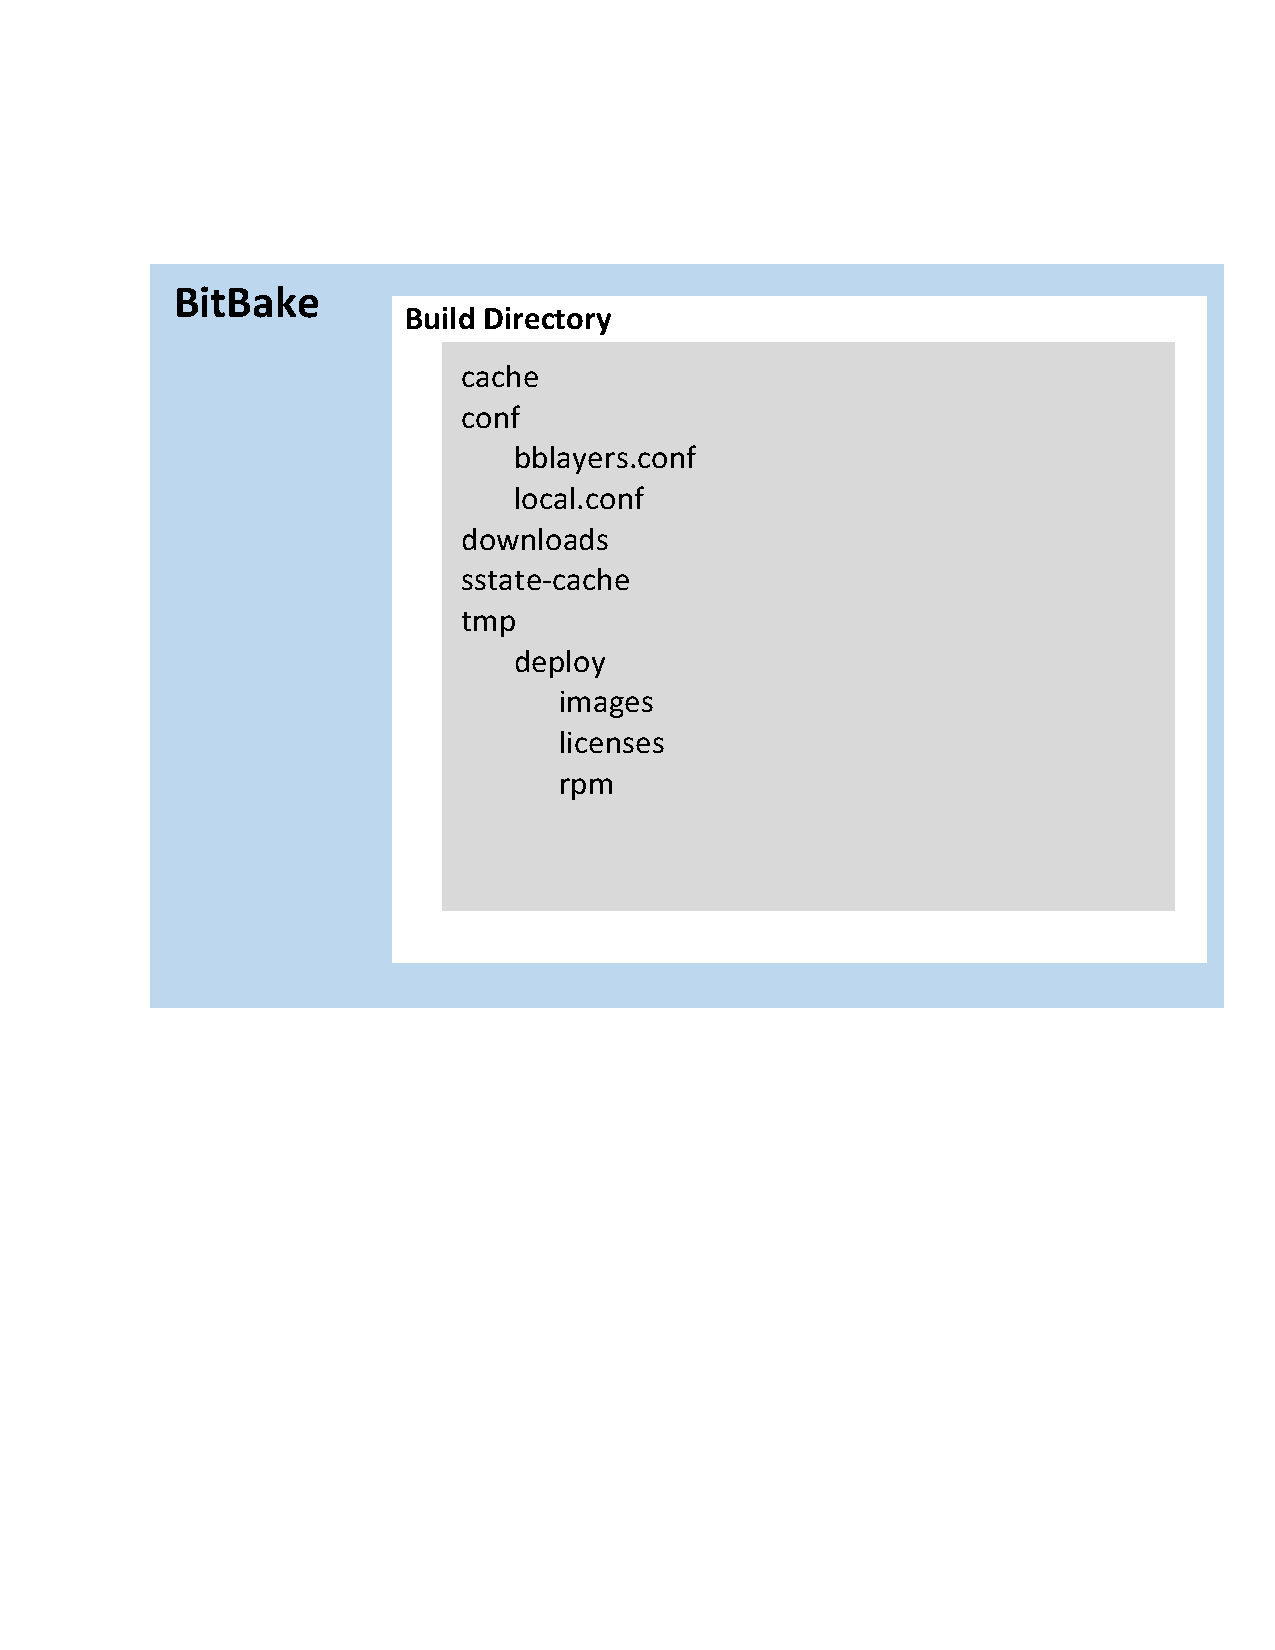
\includegraphics[width=0.7\textwidth]{figures/BitBake build directory.pdf} }}%
\caption{The Yocto Build Directory}
\label{fig:yoctobuilddir}
\end{figure}
\vspace{0.5cm}

%---------------------------------------------------------------------------------------
\subsection{Configuring the Build Directory}

The build directory contains two important user configuration files:

\begin{itemize}
 
\item{bblayers.conf} – This file contains the list of all the metadata layers which are needed by BitBake to run during the build. The file is named as \texttt{"bblayers.conf"} and is stored inside the \texttt{conf} directory within the Build Directory. The listing~\ref{lst:listing-bblayers} below illustrates a sample bblayers.conf file. Here, \texttt{YOCTO\_LAYERS} includes all the base layers predefined by the Yocto Project and essential to run the build. \texttt{EXTRA\_LAYERS} and \texttt{BOSCH\_TT\_LAYERS\_PLATFORM} denotes all the custom, user-defined layers specific to the project. 

\vspace{0.5cm}
\lstset{style=mystyle}
\lstinputlisting[caption=A bblayers.conf list all the conventional default Yocto layers and additional Bosch layers for building a custom Yocto image, captionpos=b,   basicstyle=\footnotesize, stepnumber=1, frame=lines, numbers=left, label={lst:listing-bblayers}, language=Python]{code/bblayers.conf}
\vspace{0.5cm}

Any variable set by using the "=" overrides the same variable value set elsewhere, also known as hard assignment. "?=" is the soft assignment which means the variable will not be set if defined somewhere else in the environment.


\item{local.conf} – The local configuration or the “\texttt{local.conf}” file within the build directory or precisely inside the \texttt{conf} directory stores project specific information and  parameters like selection of the target machine via \texttt{MACHINE} parameter, packages needed in the final image, types of packages (debian, rpm, ipk) and distribution to use via \texttt{DISTRO} parameters~\parencite{swain2015design}. For example, consider the following listing~\ref{lst:listing-localconf} below where a minimal local.conf file is configured for the "\texttt{poky-boschtt-systemd}" distribution for the machine type "\texttt{commodul}". \texttt{MIRRORS} and \texttt{PREMIRRORS} parameter variables for recipe source \ac{URL} redirection can also be set in the local configuration file.

\vspace{0.5cm}
\lstset{style=mystyle}
\lstinputlisting[caption=Local user settings according to the target requirements of the custom Yocto image are set in the local.conf file, captionpos=b,   basicstyle=\footnotesize, stepnumber=1, frame=lines, numbers=left, label={lst:listing-localconf}, language=Python]{code/local.conf}

\vspace{0.5cm}
\end{itemize}

One can also make use of \keyword{Hob}, a graphical user interface for BitBake by the Yocto project to set or modify the “\texttt{local.conf}” and “\texttt{bblayers.conf}” conveniently without any physical intervention to the actual file. It enables the user to select the base image type or packages needed for the target image from the \ac{GUI} itself. Hob will automatically make suitable changes in these files~\parencite{swain2015design}. 
%----------------------------------------------------------------------------------------
\subsection{Recipes} \label{section:recipes}

All the software package information is stored in the recipe file. Creating custom recipes for  target hardware is always preferable since it could be tailored to suit the exact target requirements~\parencite{swain2015design}. One can recognize a recipe file with the .bb extension. BitBake uses recipes to define how the software packages are build. Recipes contain the path to the source directory of the software packages, dependencies, instructions to compile the source files and package the compiled output~\parencite{veromannembedded}. In contrast to configuration files, the variable assignments made within the recipe are local to the recipe only~\parencite{ Reference1}. One feature offered by BitBake is sharing the common functionalities between recipes via BitBake \texttt{classes}, identified by “\texttt{.bbclass}” suffix. The classes provide base methods and are used to define the behaviour of the build system. The recipes and the classes contains code written in shell script or python code~\parencite{salvador2014embedded}. To use the functionality of a class, the recipe uses the \texttt{inherit} directive. The below listing \ref{lst:listing-recipeurl} uses the BitBake class inheritance feature, to inherit the "\texttt{packageclass}" class functionality into its recipe. Another BitBake feature is the \texttt{append} files, commonly used by layers to build on top of other layers to tweak variable settings in the recipes contained in those layers for special requirements~\parencite{Reference1}.

\subsubsection{The installation of software packages with recipes} \label{section:softwarepackageinrecipes}

In general, BitBake can execute tasks which includes shell functions written in shell scripts and BitBake style python functions. Existing class files also have predefined tasks that can be called into recipes and classes. A very special example will be the \emph{base.bbclass} which contains a set of common functionalities and is automatically included in all recipe and class files~\parencite{team2006openembedded}. One can also make use of the regular python functions inside a recipe file or class file. This section will provide a detailed overview of how BitBake executes task to build the application package with the help of recipe files. A portion of the research work also conducted by leveraging the power of the BitBake task or regular python functions. The BitBake tasks are only recognised by the recipe files (.bb) or class files (.bbclass) which are inherited from the recipe files. 

\begin{itemize}
 
\item \keyword{Fetch} - The first step of the obtaining the software package into the build environment is defining a source file path or source \ac{URL} address. Typically, it is written within the recipe (.bb) file, usually defined with the variable name "SRC\_URI". This can however be defined with other custom variable names as well. BitBake offers several download fetcher protocols like \ac{FTP} and \ac{HTTP}. The recipe file configured in the thesis work had implementations to fetch the source code of the released version of the software package from \ac{HTTP} or \ac{HTTPS} source with the help of wget fetcher and Bosch development source control management system like GIT, with the help of GIT fetcher. Remote \ac{URL} sources such as download sites or repositories are commonly supplemented with trailing patches number and auxiliary files that are stored on a local filesystem~\parencite{Reference1}. Fetching the source from remote is very flexible and easily adaptable as well. An example recipe file contains the following source \ac{URL} addresses for a software package.

\vspace{0.5cm}
\lstset{style=mystyle}
\lstinputlisting[caption=An application recipe file that potrays the concept of class inheritance and also fetch mechanism using the source \ac{URL}, captionpos=b,   basicstyle=\footnotesize, stepnumber=1, frame=lines, numbers=left, label={lst:listing-recipeurl}, language=Python]{code/recipeurl.bb}
\vspace{0.5cm}

\item \keyword{Download and Unpack} - Followed by fetching the software package source code, it is downloaded via the download() method and unpacked into a specified directory inside the \emph{WORK DIRECTORY} also referred by \texttt{WORKDIR} variable . The work directory stores extracted source package and files. Commonly, the source code is wrapped into compressed tar archives. Depending on the requirement, different compression formats can also be used.  The work directory also holds the log files and run or installation files which are generated at the time when BitBake executes recipe file.  BitBake uses multiple search methods to get the source package downloaded when it fails to access the original \ac{URL} mentioned in the recipe file. For example, fetching via \texttt{MIRRORS} and \texttt{PREMIRRORS} path variable defined in the recipe itself or \texttt{conf/local.conf}. One very important concept in the process of download and unpacking, is the checksum verification for file integrity. BitBake fetcher also verifies the checksum or hash values for archive downloads.  A “\texttt{.done}” stamp is also placed after the download is complete and checksum is verified, to avoid downloading the same source again during subsequent builds. The extracted source within the WORKDIR is usually downloaded and unpacked in the form <packagename>-<version>.

\item \keyword{Patch and Install} - Modifications to the source code is done via patching. There are various reasons why source code requires patching: adding functionalities, applying bug and security fixes, providing configuration information, or adjustments for cross-compiling~\parencite{Reference1}. Install step usually means copying source files, configuration, or binaries to user-defined target directories. It is done via the shell "\texttt{install}" command. The install utility can also set file ownership and permissions while copying the files~\parencite{Reference1}.
\end{itemize}
%----------------------------------------------------------------------------------------
\subsection{Meta-layer and metadata files}

Layers are the repositories inside the build environment. It functions like containers to group and organize recipes, classes, configuration files, and other metadata into logical entities~\parencite{Reference1}. Layers collaborate and extend each other. A build system holds multiple layers to store different software packages like \ac{BSP} layer for the hardware, \ac{GUI} layer, distribution layer required for the OS configuration, product-specific layer for required additional applications.  For example, the software package and the applications needed for a specific embedded product are mostly isolated into the product-specific layer. The advantage of layer isolation is to foster the future modifications needed according to project requirements. Figure \ref{fig:Meta layer architecture} illustrates the meta layer architecture in the OpenEmbedded Build System. A layer name is mostly prepended by a prefix “\texttt{meta-}“. The OE Core is the main base for the layer architecture. It is the main Yocto Project layer maintained by the OpenEmbedded community and by the Yocto project~\parencite[p.~150]{violanteembedded}. It contains the recipes for core software packages like the bootloaders, networking, Linux kernel and base class to build these packages, package the software with package management systems, create filesystem images, and extend the BitBake functionality~\parencite{Reference1}.
%----------------------------------------------------------------------------------------
\begin{figure}[H]
\centering
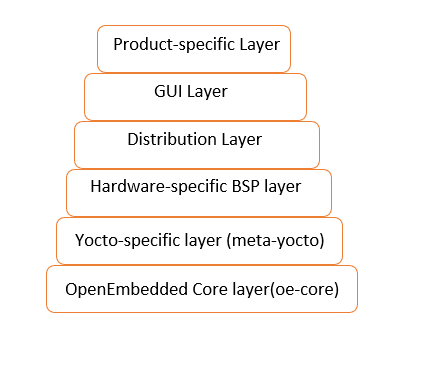
\includegraphics[scale=0.8]{figures/Layers.png}
\caption[Meta layer architecture]{Meta layer architecture.}
\label{fig:Meta layer architecture}
\end{figure}
%----------------------------------------------------------------------------------------
Metadata files are subdivided into \emph{configuration files} and \emph{recipes}~\parencite{Reference1}. BitBake uses metadata files to control the build process. Figure \ref{fig:Layer layout} shows meta- layer directory tree and its subdirectory files. The \texttt{conf} subdirectory have the layer configuration file \texttt{layer.conf} which identifies the file structure as a layer, contents of the layer and instructions about how the build system should use it~\parencite{Reference2}. Each layer has its own \texttt{layer.conf}.
%----------------------------------------------------------------------------------------
\vspace{0.5cm}
\begin{figure}[H]
  \centering 
\begin{forest}
  pic dir tree,
  where level=0{}{% folder icons by default; override using file for file icons
    directory,
  },
  [meta-<layername>
    [classes
        [aclass.bbclass, file]
        [bclass.bbclass, file]
    ]
    [conf
        [layer.conf, file]
    ]
    [machine
        [amachine.conf, file]
    ]
    [distro
      [distro.conf, file]
    ]
    [recipe-<a category>
        [<package 1>
            [<package1>\_<version>.bb, file]
        ]
        [<package 2>
            [<package2>\_<version>.bb, file]
        ]
    ]
    [recipe-<b category>
      [<package 1>
            [<package1>\_<version>.bb, file]
        ]
        [<package 2>
            [<package2>\_<version>.bb, file]      
      ]
    ]
  ]
\end{forest}
\caption{Layer layout}\label{fig:Layer layout}
\end{figure}

%----------------------------------------------------------------------------------------
\newpage
\subsection{Images} 

The images  are  essentially configured  packages that generate a filesystem~\parencite{veromannembedded}. The final aim of developing a custom Linux distribution and the build process is the target image. The bootable image can then be flashed on the hardware. Final images are placed inside the image folder within the deploy  directory.  One can also make use of reference pre-made image that Poky distribution offers and implement custom images from it.  This work also implemented a custom Linux distribution using the reference “\texttt{core-image-minimal}” image which Poky offers.

One can also use other Poky distribution reference images. The “core-image-full-cmdline” for console-only image,with full functionality of featured Linux system. or “\texttt{core-image-x11}" image for a basic \ac{GUI} experience~\parencite{veromannembedded}. 
  
%----------------------------------------------------------------------------------------
\section{Summary}



\clearpage\null\thispagestyle{empty}

